\documentclass{sigchi}

% Remove or comment out these two lines for final version
\toappearbox{\Large Submitted to CHI'13. \\Do not cite, do not circulate.}
\pagenumbering{arabic}% Arabic page numbers for submission. 

% Use \toappear{...} to override the default ACM copyright statement (e.g. for preprints).

% Load basic packages
\usepackage{balance}  % to better equalize the last page
\usepackage{graphics} % for EPS, load graphicx instead
\usepackage{times}    % comment if you want LaTeX's default font
\usepackage{url}      % llt: nicely formatted URLs
\usepackage{caption}
\usepackage{subcaption} 
\usepackage{amssymb}
\usepackage{amsmath}

% llt: Define a global style for URLs, rather that the default one
\makeatletter
\def\url@leostyle{%
  \@ifundefined{selectfont}{\def\UrlFont{\sf}}{\def\UrlFont{\small\bf\ttfamily}}}
\makeatother
\urlstyle{leo}


% To make various LaTeX processors do the right thing with page size.
\def\pprw{8.5in}
\def\pprh{11in}
\special{papersize=\pprw,\pprh}
\setlength{\paperwidth}{\pprw}
\setlength{\paperheight}{\pprh}
\setlength{\pdfpagewidth}{\pprw}
\setlength{\pdfpageheight}{\pprh}

% Make sure hyperref comes last of your loaded packages, 
% to give it a fighting chance of not being over-written, 
% since its job is to redefine many LaTeX commands.
\usepackage[pdftex]{hyperref}
\hypersetup{
pdftitle={SIGCHI Conference Proceedings Format},
pdfauthor={LaTeX},
pdfkeywords={SIGCHI, proceedings, archival format},
bookmarksnumbered,
pdfstartview={FitH},
colorlinks,
citecolor=black,
filecolor=black,
linkcolor=black,
urlcolor=black,
breaklinks=true,
}

% create a shortcut to typeset table headings
\newcommand\tabhead[1]{\small\textbf{#1}}


% End of preamble. Here it comes the document.
\begin{document}

\title{SIGCHI Conference Proceedings Format}

% Note that submissions are blind, so author information should be omitted
\numberofauthors{3}
\author{
  \alignauthor 1st Author Name\\
    \affaddr{Affiliation}\\
    \affaddr{Address}\\
    \email{e-mail address}\\
    \affaddr{Optional phone number}
  \alignauthor 2nd Author Name\\
    \affaddr{Affiliation}\\
    \affaddr{Address}\\
    \email{e-mail address}\\
    \affaddr{Optional phone number}    
  \alignauthor 3rd Author Name\\
    \affaddr{Affiliation}\\
    \affaddr{Address}\\
    \email{e-mail address}\\
    \affaddr{Optional phone number}
}

% Teaser figure can go here
%\teaser{
%  \centering
%  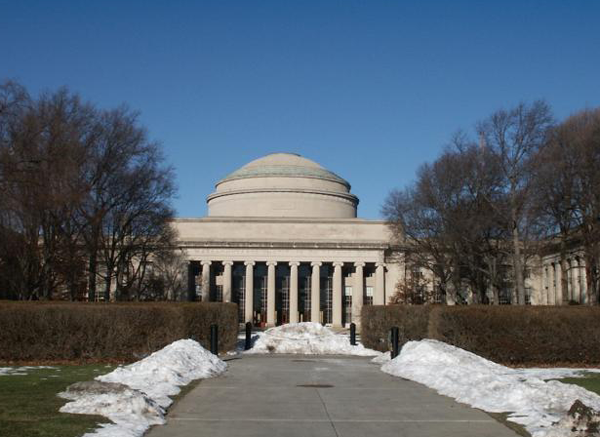
\includegraphics{Figure1}
%  \caption{Teaser Image}
%  \label{fig:teaser}
%}

\maketitle

\begin{abstract}
Handwriting recognition is a natural and versatile method for data
entry, especially on mobile devices and devices with touch
screens. However, as handwriting is highly variable, it is difficult
to design handwriting recognizers that perform well for everyone. A
natural solution is to use machine learning to adapt the recognizer to
the user. One complicating factor is that, as the computer is adapting
to the user, the user is also adapting to the computer. The
contributions of this paper are in three complementary
directions. First, we devise an information-theoretic framework for
quantifying the efficiency of a handwriting system where the system
includes both the user and the computer. From this framework, we
derive two performance measures that are used to gamify handwriting
adaptation. Second, we develop and deploy an adaptive handwriting
recognition system in the context of a game that runs on iOS
devices. Finally, we perform a statistical analysis of the system’s
performance on the data collected from 15 different users over
multiple sessions and characterize the impact of machine adaptation
and of human adaptation.
\end{abstract}

\keywords{
	Guides; instructions; author's kit; conference publications;
	keywords should be separated by a semi-colon.
	\\\textcolor{red}{Mandatory section to be included in your final version.}
}

\category{H.5.m.}{Information Interfaces and Presentation (e.g. HCI)}{Miscellaneous
\\
\textcolor{red}{See: \url{http://www.acm.org/about/class/1998/}
for more information and the full list of ACM classifiers and descriptors. 
Mandatory section: On the submission page
only the classifiers' letter-number combination will need to be entered.}
}

\terms{
	Human Factors; Design; Measurement. 
	If you choose more than one ACM General Term, 
	separate the terms with a semi-colon.
\\
\textcolor{red}{If you choose more than one ACM General Term, 
separate the terms with a semi-colon. See list of ACM terms at:
\url{http://www.sheridanprinting.com/sigchi/generalterms.htm}.
Optional section to be included in your final version.}
}

\section{Introduction}

There is a large asymmetry in human-computer interfaces. The computer
to human channel has a much higher bandwidth than the human to
computer bandwidth. With the progress of computers with small form
factor such as smart phones and tablets, this limitation is becoming
increasingly problematic.

The most common approach for entering textual information on a smart
phone is soft-keyboard where input rates of around 20 - 25 words
per minute (WPM) have been reported\cite{Arif2009,
  Castellucci2011}. These rates are for English. For languages with
larger number of characters such as Thai (49 characters), Japanese or
Chinese (hundreds to thousands of letters, depending on the context),
soft-keyboard becomes impractical. Even when using English, the need
to use digits or special characters "!?\&\$\#\@\;\:\,\." can
significantly decrease the typing speed.

\newcommand{\tm}{\textsuperscript{\textregistered}~}

Many alternatives to the standard soft-keyboard exist. For example,
Swype\tm provides a method for tracing a path between keyboard keys
and lifting the finger from the screen at the end of each
word. TikiNotes\tm uses a keyboard with 9 large keys, each
corresponding to several letters or an auto-completion
alternative. Dasher~\cite{Garrett2003} is a particularly innovative
method where typing is replaced by using a joystick-like pointer to
fly through clouds of characters. Finally, there are handwriting
recognition software that allow the user to enter information using
natural handwriting.

A user of any one of these methods typically improves significantly
with practice. There are many competitions between different data
entry methods. However, these comparisons are inherently flawed in
that the contender is always a person who can enter information faster
than the current record holder, most likely as a result of extensive
training. In other words, {\em user adaptation} cannot be ignored.

To evaluate the efficacy of a particular data entry method it is
therefore necessary to measure the performance of each user over a
sufficiently long period of time so that the performance of the user
stabilizes. As we are interested in machine learning methods we arrive
at the interesting situation in which both the computer and the human
adapt over time in an effort to maximize the input rate of the
data entry method. We refer to this situation as {\em co-adaptation}.
 

% \iffalse
% A natural way to measure the speed of data entry is to count the
% number of letters entered correctly per second. However, this puts too
% large a penalty on mistakes. Suppose a user intends to write the
% letter $h$ but enters a letter than looks more like the letter
% ``n''. We can count this as a mistake. However, if the recognition
% algorithm gives 50\% probability to ``n'', 40\% probability to the
% letter ``h'' and less than 1\% probability to the other 24 letters,
% then we can say that the user did provide significant information
% about the intended letter. Combining this information with information
% on inter-character dependence can be used to resolve the ambiguity.
% \fi


Handwriting data is usually analyzed one ``unit'' at a time where
``unit'' can be a stroke, a chracter, a word or even a
sentence. In this work, we propose an alternative analysis where the
data is analyzed in fixed intervals of time. We consider the process
of writing as a process of through which the intended letter is
disambiguated from the other possible letters. 



In this paper we focus on handwriting recognition systems where a user
sends the information, one character at a time, to the computer using
her natural handwriting. To quantify the rate of information
transmitted, we compute the mutual information between the intended
character and the decoded character distribution and divide it by the
length of time it takes to complete writing the letter. This ratio
defines the data rate in the information theoretic sense.  The exact
definition will be given in Section~\ref{sec:channel}.


% \iffalse
% The contributions of this paper are:
% \begin{itemize}
% \item A theoretical framework for quantifying the data transfer rate
%   of a system that combines a human writer and a handwriting
%   recognition system.
% \item An adaptive handwriting recognition system that is based on
%   unsupervised clustering and Bayesian inference.
% \item Results from a small deployment of the system, demonstrating
%   its promise.
% \item A method for visualizing the process by which the identity of
%   the character is decoded in continuous time leading to suggestions
%   for how to improve the handwriting of the user. 
% \end{itemize}
% \fi

The paper is organized as follows. In Section~\ref{sec:channel}, we
describe the handwriting channel and define the information rate. In
Section~\ref{sec:recognition_algorithm}, we present our recognition
algorithm. In Section~\ref{sec:experiment} and
Section~\ref{sec:results}, we describe the experiment and present the
results respectively. Finally, we draw some conclusions in
Section~\ref{sec:conclusions}.

\section{Handwriting recognition as a communication channel}
\label{sec:channel}

Unlike typing, which transmits information to the computer at discrete
time points, handwriting has to be described as a continuous time
process. We can describe the process as a communication channel in
continuous time as depicted in Figure~\ref{fig:hwr_channel}.

% input
\newcommand{\intent}{M}
\newcommand{\intentSet}{\mathcal{E}}
\newcommand{\intentDist}{\mathcal{M}}
% output
\newcommand{\pred}[1]{\mathcal{Q}_{#1}}
\newcommand{\predFinal}{\pred{final}}
% trajectory
\newcommand{\writing}[1]{W_{1:{#1}}}
\newcommand{\writingDist}{P(\bar{W} | \intent)}
% misc
\newcommand{\tFinal}{T}
\newcommand{\MI}{I(\intent ; \predFinal)}
\newcommand{\EMI}{\hat{I}(\intent ; \predFinal)}
\newcommand{\session}{\mathcal{S}}
\newcommand{\bps}{R}
\newcommand{\logloss}{\mathcal{L}}
\newcommand{\expectedDuration}{\mathbb{E} \left[\tFinal\right]}

We formalize this process using the concept of a communication
channel~\cite{Shannon1948}.  Let $\intentSet$ denote the set of all
possible input. Technically, $\intentSet$ can be a set of sentences, a
set of words, or a set of characters depending on the designed of the
handwriting recognition system. Without loss of generality, we assume
that $\intentSet$ is a set of 26 English characters and ignore
dependencies between characters due to the language model or due to
the co-articulation effects between neighboring handwritten
characters.

As shown in Figure~\ref{fig:hwr_channel}, the channel is comprised of
two separate processes. First, the handwriting process is the process
of which the user translates an intent $\intent$ into a series of hand
movements which is sampled at some rate to create a discrete time
trajectory: $\writing{T} = \left[ (x_1,y_1), \ldots, (x_T,y_T)
\right]$. In other words, this process {\em encodes} the intent
$\intent$ into a trajectory $\writing{T}$. We can model the
variability in the encoding with the distribution $\writingDist$. The
second process is the process of decoding the handwriting trajectory
into the original intent. For each time step $1 \le t \le T$, the process
maps a trajectory $\writing{t}$ to a distribution over $\intentSet$,
$\pred{t}$, which is also the output of the channel.

\begin{figure}
  \centering
  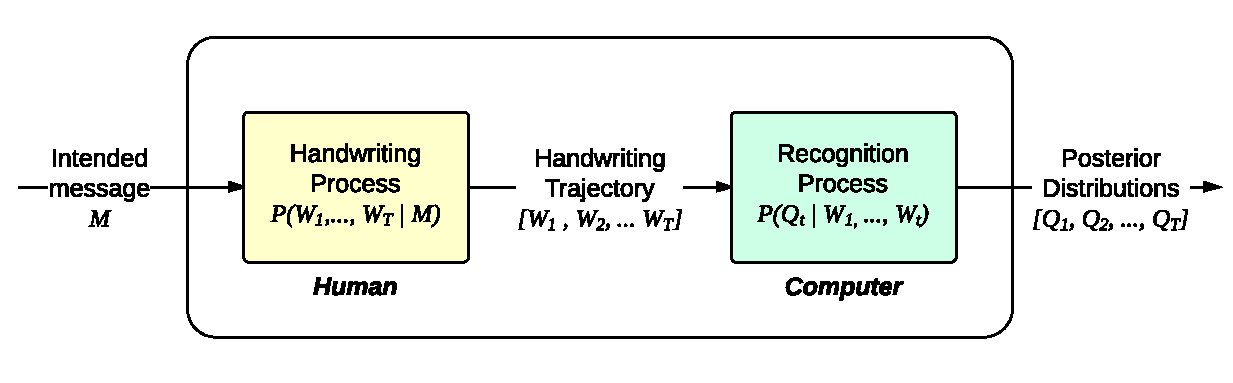
\includegraphics[width=0.9\columnwidth]{figures/hwr_channel.pdf}
  \caption{A summary of the handwriting recognition channel.}
  \label{fig:hwr_channel}
\end{figure}

Let $\tFinal$ and $\predFinal$ denote the time and the posterior
distribution when the user finishes writing the input respectively.
According to the theory of channel capacity, the information
transmitted through the channel by the time the user completes writing
the character is quantified by the mutual information between the
input $\intent$ and the decoding posterior $\predFinal$, $I(\intent ;
\predFinal)$. We now unpack this expression.  We define the mean
posterior of $\predFinal$ conditioned on $\intent$ and the average
posterior distribution as follows.
\[
P(\predFinal | \intent)=
\sum_{\bar{w} \sim \writingDist} { P(\predFinal | \writing{\tFinal} = \bar{w})
P(\writing{\tFinal} = \bar{w} | \intent)} 
\]
\[
P(\predFinal)
=
\sum_{m \in \intentSet} 
P(\intent = m) P(\predFinal | \intent = m)
\]
Given these two expressions, we can define the mutual information
between the character $\intent$ and the decoding $\predFinal$ to be 
\[
I(\intent ; \predFinal) = H(\predFinal) - \sum_{m \in \intentSet})
P(\intent = m) H(\predFinal | \intent)
\]
where the entropy of $\predFinal$ is defined as
\[
H(\predFinal) = -\sum_{m in \intentSet} {
P(\predFinal = m) \log_2 P(\predFinal = m)}
\]
Now we define the channel rate to be 
\begin{align}
\label{eq:channel_rate}
R_{MI}(\intent, \predFinal) 
= 
\frac{I( \intent ;  \predFinal)}{\expectedDuration}
\end{align}

The channel rate $R_{MI}$ yields a high value as long as $P(\predFinal |
\intent)$ concentrates on some intent. We propose another measure of
the channel rate $R_{logloss}$ based on the idea of log loss that
also penalizes incorrect concentration.
\[
R_{logloss}(\intent, \predFinal)
=
\frac{H(\predFinal) - \sum_{m \in \intentSet})
P(\intent = m) L(\predFinal | \intent)}{\expectedDuration}
\]
where
\[
L(\predFinal | \intent) 
=  
\sum_{m \in \intent} P(\intent = m) [ - \log_2 P(\predFinal = m |
\intent = m) ]
\]

\begin{enumerate}
\item $R_{MI} \ge R_{logloss}$ when $P(\predFinal = m | \intent =m) < 1/|\intentSet|$ 
because $\mathcal{E}[-\log_2 P(\predFinal | \intent = m)] \le \log_2
|\intentSet|$ and $\log_2 |\intentSet| \le -\log_2 P(\predFinal = m |
\intent = m)$\\
\item $R_{logloss} \ge R_{MI}$ when $P(\predFinal = m | \intent =m)
  \ge \mathcal{E}_j[P(\predFinal = j | \intent = m)]$ since $-\log_2
  P(\predFinal = m | \intent =m) \le -\log_2
  \mathcal{E}_j[P(\predFinal = j | \intent = m)] \le \mathcal{E}_j[
  -\log_2 P(\predFinal = j | \intent = m)]$ 
\end{enumerate}

Intuitively, the channel rate is a measure that quantifies both
accuracy and speed of a handwriting recognition channel at the same
time. Handwriting, as well as many other motor control tasks, obeys
the speed-accuracy tradeoff~\cite{Fitts1954}. It is not sufficient to
quantify the efficiency of a handwriting recognition system by its
recognition accuracy alone. For example, a system that requires the
user to write each character in a specialized form may attain a very
high recognition accuracy, but it would require the user more time and
effort to use. Such system might not be as efficient as a system that
makes more errors but allows the user to write freely. In a sense,
maximizing the channel rate is equivalent to finding a balance between
maximizing the recognition accuracy and minimizing the writing time
and effort of the user.

Based on the model, we suggest that the channel rate can be improved
by a combination of human learning and machine learning, which
corresponds to improving the handwriting process and the recognition
process respectively. Ideally, $\predFinal$ is always concentrated
on the original intent $\intent$. This would mean that the channel is
perfect and works without error. However, in real-world scenarios,
errors will occur. One source of errors comes from misrecognition in
the recognition process. These recognition errors can be reduced using
training data and machine learning. The harder problem is when there
is a significant overlap between $\writingDist$ for different
intents. In this situation, we need to rely on the user to make
their handwriting less ambiguous. Although the effect of human
learning is always present, we believe that it can be enhanced by
giving useful feedback to the user in the form of guidance or lessons.


\section{Adaptive recognition algorithm}
\label{sec:recognition_algorithm}

We developed an adaptive single-character recognition algorithm for
translating the handwriting trajectory $\writing{t}$ to one of the
characters in $\intentSet$. By realizing that the effect of user
adaptation can always be present, we designed our recognition
algorithm to be able to handle the fact that the handwriting
trajectory distribution $\writingDist$ can be different at
different time $t$. The idea of specializing and adapting the
recognizer for each user has been studied and shown to be effective in
reducing the error rate~\cite{Connell2002, Matic93, Kienzle06}.

At a high-level, our recognition algorithm can be described as
follows. For each user, the algorithm creates and maintains one or
more Markov-based models~\cite{ThomasPloetz2011} for each of the
characters. We refer to each model as a {\em prototype}. The adaptivity
of our algorithm comes from the re-training of the prototype set. In
the decoding step, at each time step $t$, the algorithm calculates the
likelihood of each character. The character with the highest
likelihood is predicted. In addition, for our analysis, it also
outputs the posterior probability distribution over the characters
$\predFinal$.

\subsection{Prototype training}

For each character $c \in \intentSet$, our aim is to discover
different writing styles of $c$ and create a prototype for each of
them. To do so, we perform a hierarchical clustering with the {\it
  dynamic time warping} (DTW) distance~\cite{Rabiner1993} on a set of
handwriting instances. Each handwriting instance is described by a
sequence of feature vectors $\langle f_1, \ldots, f_T \rangle$ where
$f_i = (x_i,y_i, dx_i,dy_i)$.  $(x_i,y_i)$ denotes the normalized
touchscreen coordinate and $(dx_i,dy_i) = (\frac{x_i - x_{i-1}}{z},
\frac{y_i - y_{i-1}}{z}) , z = \sqrt{(x_i - x_{i-1})^2 + (y_i -
  y_{i-1})^2}$ denotes the writing direction.

Once the cluster structures are found, for each cluster, we find the
medoid of the cluster and transform it into a prototype i.e. a
left-to-right HMM with Gaussian observations. The transformation is
straightforward where each hidden state corresponds to each sampled
point in the trajectory. However, this transformation often yields a
HMM with too many hidden states than necessary. We perform an additional
step to reduce the number of hidden states by a series of removing and
merging hidden states using a variant of forward-backward
algorithm. Figure~\ref{fig:state_reduction} shows the hidden states
before and after the reduction step.

\begin{figure}[h]
  \centering
  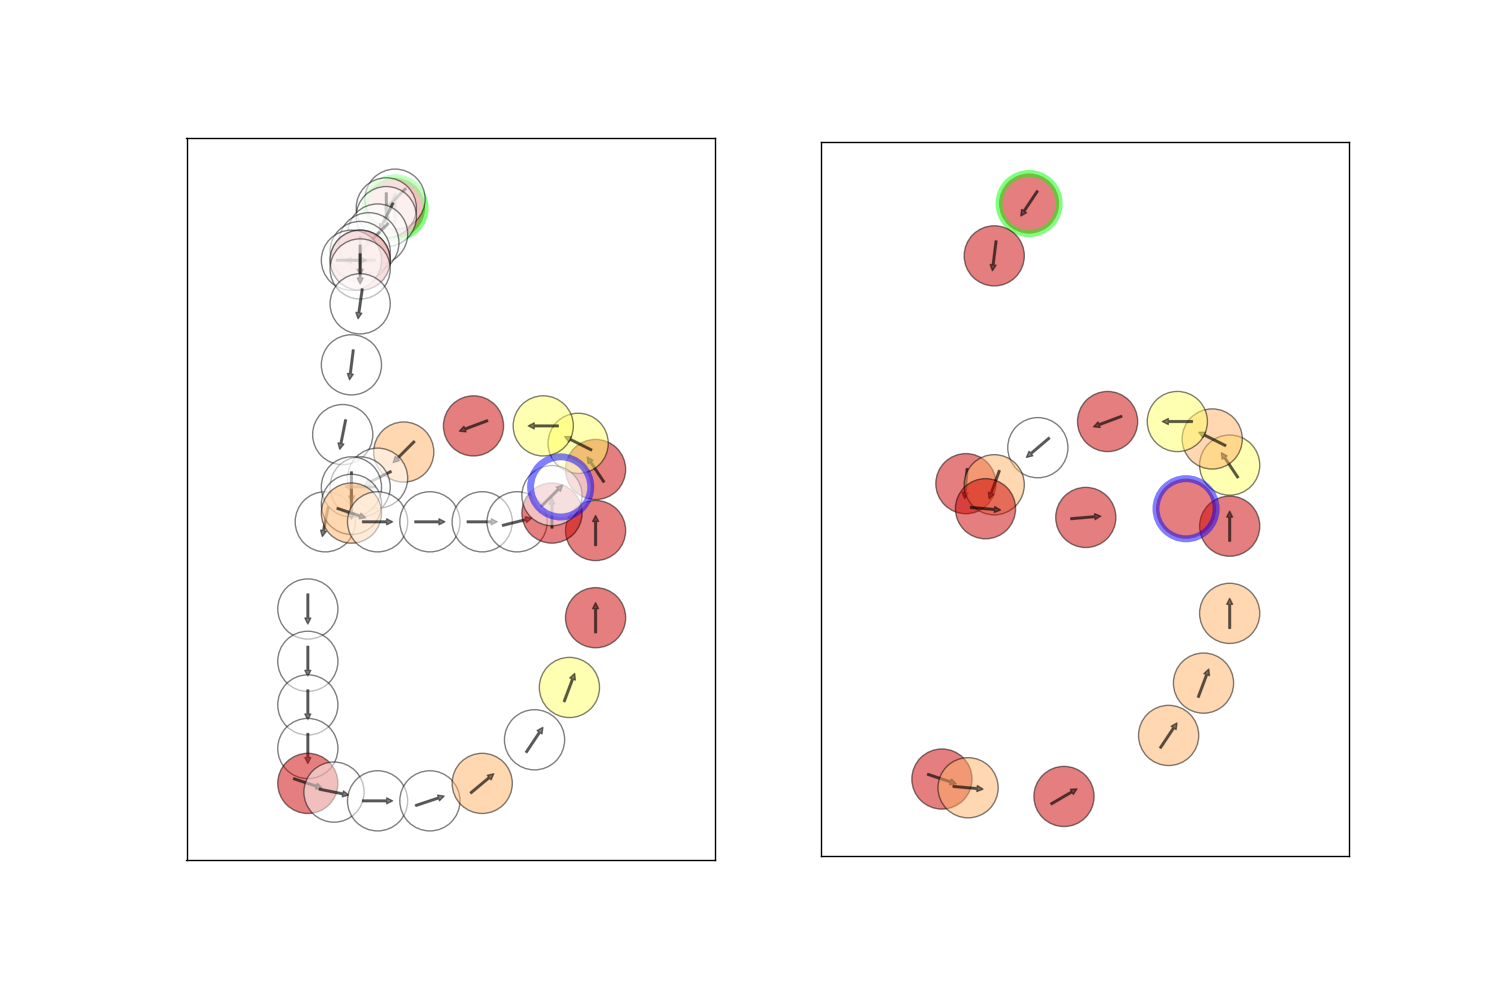
\includegraphics[width=0.5\textwidth] {figures/state_reduction.png}
  \caption{The hidden state reduction process is applied to each
    prototype to remove rarely visited states with respect to the
    training set. The originally trained prototype is shown on the
    left and the reduced prototype is shown on the right. The
    intensity of the colors corresponds to the expected number of
    times the state being mapped to. }
  \label{fig:state_reduction}
\end{figure}

\newcommand{\prototypeSet}{\mathcal{P}}

From the collection of all prototypes $\prototypeSet_{all}$, we then
select a subset of prototypes $\prototypeSet_u \subset
\prototypeSet_{all}$ for each user $u$ such that the recognition error
on the user-specific validation data with respect to $\prototypeSet_u$
is minimized. For our dataset, we found that, at most 2
prototypes are sufficient for each user-character pair. Similarly, a
prototype set for all users (writer-independent) can be found by
replacing the user-specific training data with the data from all users.

% \iffalse
% \begin{algorithm}[p]
% \caption{Prototype selection}
% \algsetup{linenosize=\tiny}
% \label{alg:selection}
% \begin{algorithmic}[1]
% \REQUIRE{$\mathcal{D}_u$ = Training set from user $u$, 
%   $\prototypeSet_{all}$ = Available prototype set}
% \STATE $\prototypeSet_u = \emptyset$
% \REPEAT
% \STATE $err \leftarrow error\_rate(\mathcal{D}_u, \prototypeSet_u)$
% \FOR{each prototype $T_{i} \in \prototypeSet_{all}$}
% \STATE $err' \leftarrow error\_rate(\mathcal{D}_u, \prototypeSet_u \cup
% \{ T_{i} \})$
% \IF{$err - err' > best\_reduction$}
% \STATE $best\_reduction \leftarrow err - err'$
% \STATE $next\_prototype \leftarrow T_{i}$
% \ENDIF
% \ENDFOR
% \STATE $\prototypeSet_u \leftarrow \prototypeSet_u \cup \{ next\_prototype\}$
% \UNTIL{$best\_reduction < \epsilon$}
% \end{algorithmic}
% \end{algorithm}
% \fi

\subsection{Decoding}

\newcommand{\forwardprob}{\alpha^{(t)}_{i,j}}

Our decoding is based on the standard Bayesian inference.
For user $u$, the algorithm maintains a set of prototypes
$\prototypeSet_u = \{ T_1, T_2, ... , T_m\}$. The probability distribution over all
the prototypes and all the hidden states of each prototype given the
handwriting trajectory $\writing{T}$, or $P(T_{i,j} |\writing{T})$, is
estimated using forward algorithm. Let $\forwardprob$ denote $P(T_{i,j} |
\writing{T})$. Based on $\forwardprob$, the probability of prototype
$T_i$ conditioned on $\writing{T}$ is given by $P(T_i | \writing{T}) = \sum_{j}
\forwardprob$. 

% \iffalse
% \begin{algorithm}[p]
% \caption{Beam-search forward algorithm}
% \label{alg:forward}
% \begin{algorithmic}[1]
% \REQUIRE{$\{T_1,..T_m\}$  = the prototype set\\ $K$ =
%   beam width \\ $A_{i,j,k}$ = the transition probability from state
%   $j$ to state $k$ of prototype
%   $T_i$ \\ $B_{i,j}(f_t)$ = the emission probability of state
%   $j$ of prototype $T_i$ with observation $f_t$}
% \STATE $\alpha^{(0)}_{i,1} \leftarrow$ the prior probability of
% prototype $T_i$
% \STATE $active \leftarrow \{ \alpha^{(0)}_{i,0} ; \forall \; 1 \le i \le m \}$
% \FOR{each time step $t$}
% \STATE $new\_active \leftarrow \{\}$
% \WHILE{$active \ne \emptyset$}
% \STATE remove $\alpha^{(t-1)}_{i,j}$ from $active$
% \FOR{$0 \le k \le 2 $}
% \STATE $\alpha^{(t)}_{i,j+k} \leftarrow \alpha^{(t-1)}_{i,j} A_{i,j,j+k} B_{i,j+k}(f_t)$
% \STATE insert $\alpha^{(t)}_{i,j+k}$ to $new\_active$ or add to the existing value
% \ENDFOR
% \ENDWHILE
% \STATE $active \leftarrow top\_states(new\_active,K)$
% \ENDFOR
% \end{algorithmic}
% \end{algorithm}
% \fi

\section{Experiment}
\label{sec:experiment}

% \iffalse
% The user interface that we use in our experiments is presented to the
% user in the form of a simple game. The user is presented with a
% sequence of characters, one character at a time. When the user sees
% the character, her goal is to write it on the touch screen as quickly
% and as legibly as possible. The computer then classifies the character
% and assigns a score to the user, based on the writing speed and on the
% legibility.
% \fi

We conducted an experiment in the format of a game where the
participants were asked to compete in a writing game. In each session,
each participant was presented with a random permutation of the 26
lowercase English alphabets i.e. $\intentSet = \left[ a \ldots z \right]$
and $P(\intent)$ is uniform. The objective of the game was to write
the presented characters as quickly as possible and, more importantly,
the handwritten characters should be recognizable by the system. A
score, which is a function of {\it channel rate}, was given to the
user right after each session to reflect the performance of the
session. There were 9 participants in this experiment. Each participant was
asked to play the writing game, which is an implementation our adaptive
recognition algorithm on Apple iPads, for at least
20 sessions over multiple days in his/her own pace. 

Prior to the experiment, we trained a prototype set $\prototypeSet_0$
with a small set of handwriting data provided by the authors. We did
not expect $\prototypeSet_0$ to work well for every user but it is
sufficient as a starting point. Let $\prototypeSet_{(u,i)}$ denote the
prototype set for user $u$ in session $i$. For every user $u$,
$\prototypeSet_{(u,1)}$ was initialized to $\prototypeSet_0$. During
the experiment, the system frequently updated the prototype set
$\prototypeSet_{(u,i+1)}$ using user-specific data collected from
previous sessions. The update happened every 2-5 sessions
depending on the availability of the training server. 

% \iffalse
% \begin{figure}
%   \centering
%   \includegraphics[width=0.3\textwidth] {figures/uright3.png}
%   \label{fig:screen_shots}
%   \caption{GUI of the writing game on Apple iPad.}
% \end{figure}
% \fi

\section{Results}
\label{sec:results}

The experiment was set up to demonstrate a condition called {\em
  co-adaptation} where both the user and the computer were allowed to
adapt together. We denote this condition $R_{adapt}$. The average
channel rates per session of each user using are shown in
Figure~\ref{fig:channel_rate_adapt}. 

To investigate the effect of co-adaptation, we create another
condition called $R_{fixed}$ where the computer was not allowed to
adapt. In other words, we ran a simulation to figure out what the
channel rates would have been if the prototype sets were never changed
from $\prototypeSet_0$. The results are shown in
Figure~\ref{fig:channel_rate_fixed}.

Although the prototype set was not changing in $R_{fixed}$, we observe
that channel rate increases over the sessions. The paired t-test
indicates a significant difference between the average channel rate in
the first 5 sessions and the average channel rate in the last 5
sessions ($p < 0.001$). This suggests that the users improve the
handwriting on their own. We call this effect {\em user
  adaptation}. 

In Figure~\ref{fig:channel_rate_per_user}, we compare $R_{adapt}$ and
$R_{fixed}$ for each user. We found that the channel rate of
$R_{adapt}$ is significantly higher than that of $R_{fixed}$ with $p = 0.007$.
This result confirms that the computer adaptation helps improving the
overall channel rate. In addition, we calculate the theoretical
maximum of the channel rate under the assumption of the perfect
recognition, denoted by $R_{ideal}$. The maximum rates are given by
$H(\character) / \expectedDuration$. In our case, $H(\character) =
\log_2(26)$. 

\begin{figure}
  \centering
  \begin{subfigure}[b]{0.3\textwidth}
    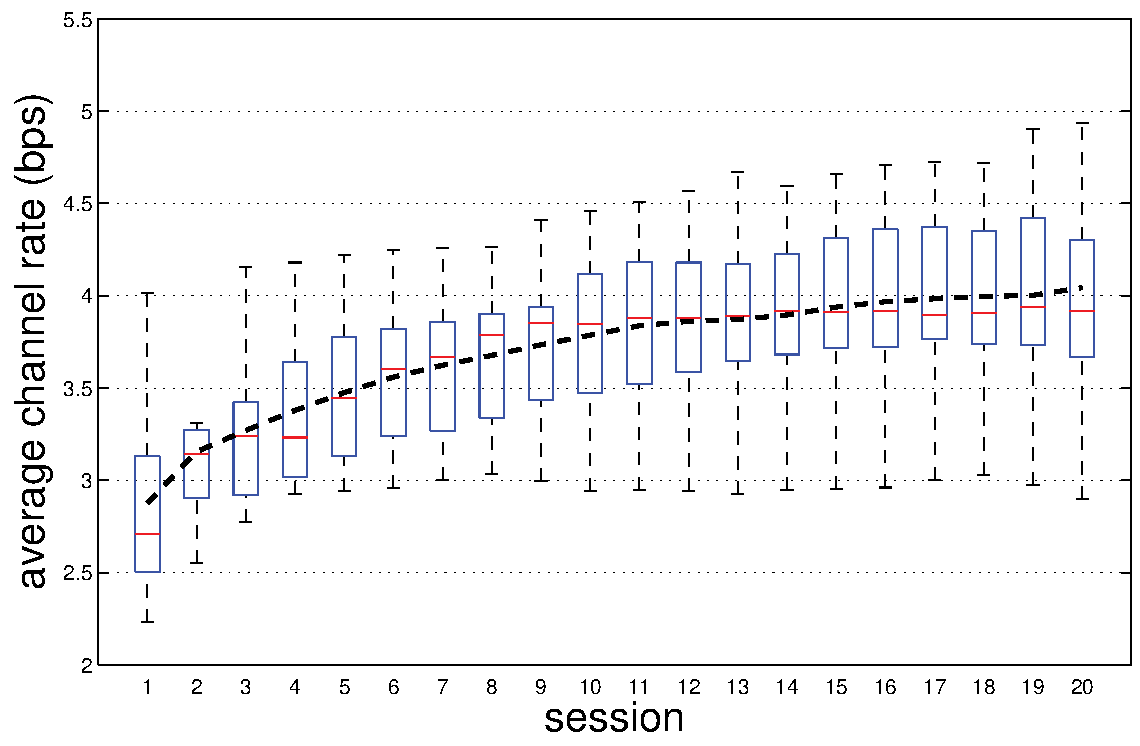
\includegraphics[width=\textwidth]{figures/IUI_BPS_p_adapt.pdf}
    \caption{$R_{adapt}$}
    \label{fig:channel_rate_adapt}
  \end{subfigure}
  \begin{subfigure}[b]{0.3\textwidth}
    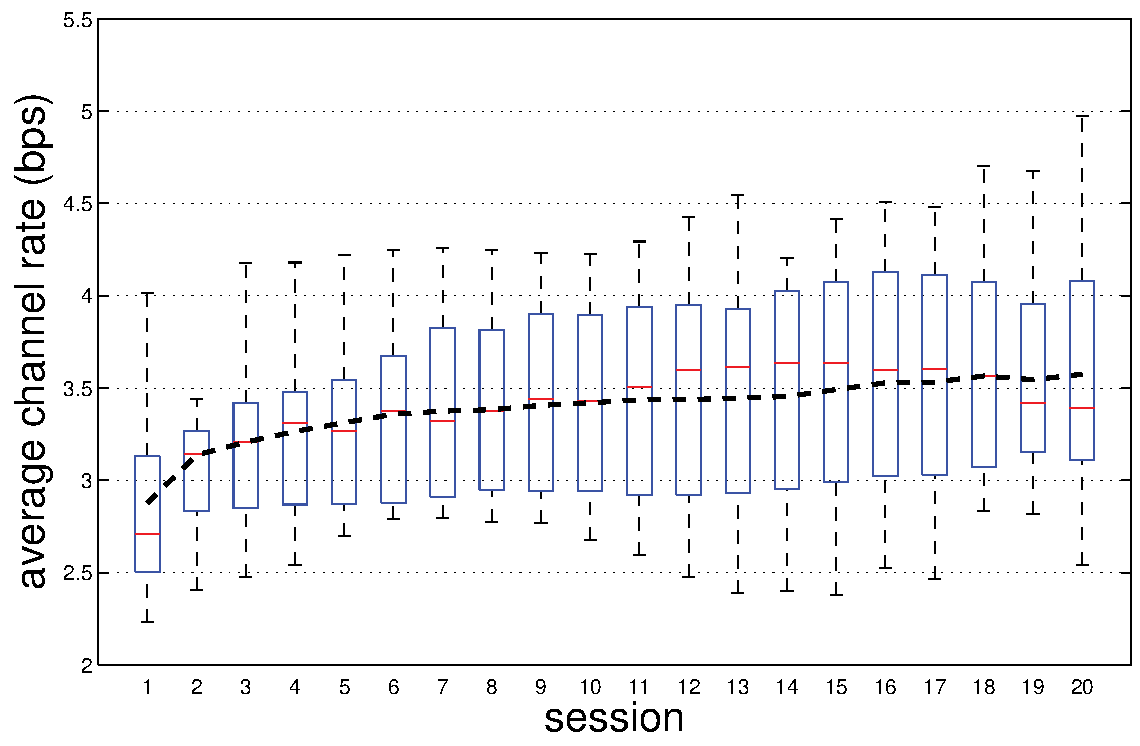
\includegraphics[width=\textwidth]{figures/IUI_BPS_p_first.pdf}
    \caption{$R_{fixed}$}
    \label{fig:channel_rate_fixed}
  \end{subfigure}
  \begin{subfigure}[b]{0.3\textwidth}
    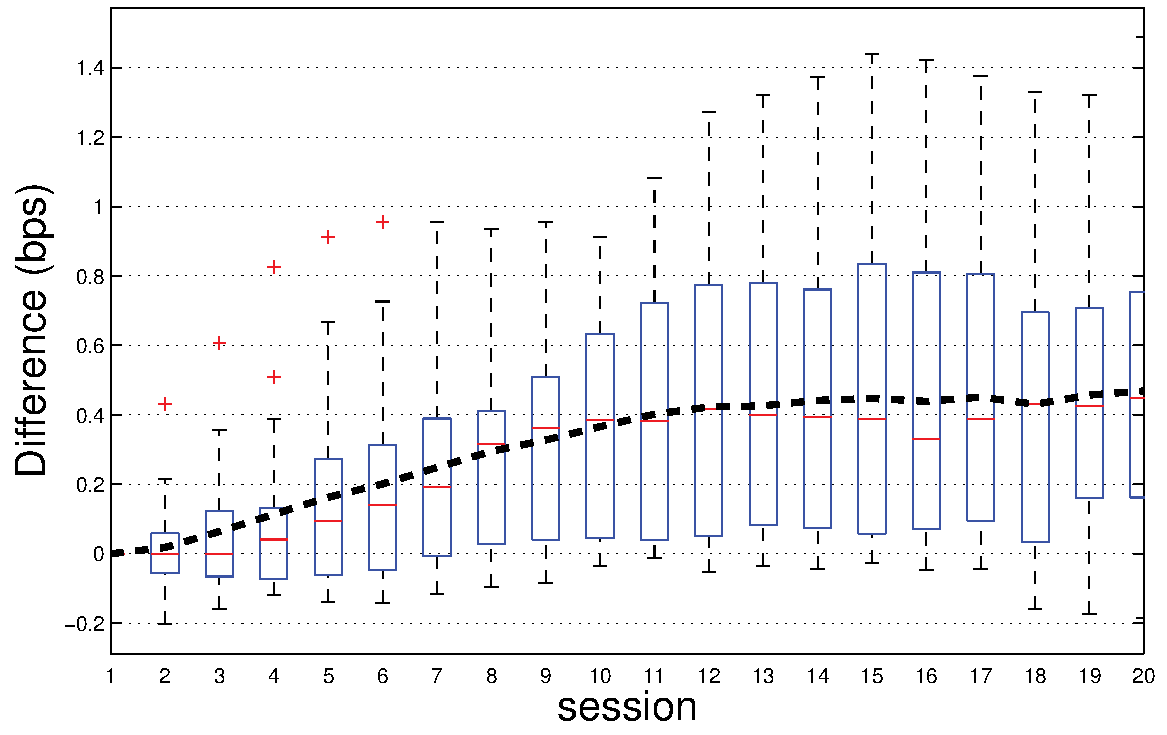
\includegraphics[width=\textwidth]{figures/IUI_BPS_diff_p_first.pdf}
    \caption{$R_{adapt} - R_{fixed}$}
    \label{fig:channel_rate_diff}
  \end{subfigure}
  \label{fig:channel_rate}
  \caption{Channel rate per session of each user with
    (\ref{fig:channel_rate_adapt}) and without (\ref{fig:channel_rate_fixed})
    presence of machine learning. }
\end{figure}

\begin{figure}
  \centering
  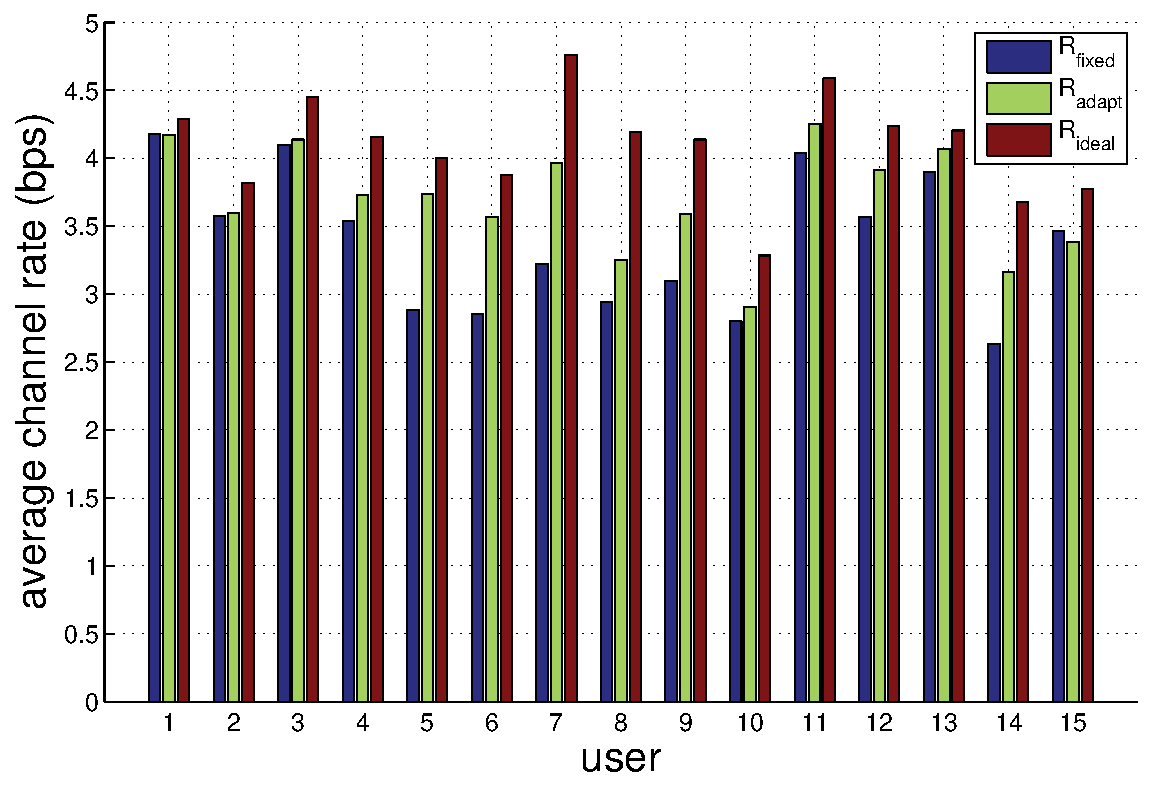
\includegraphics[width=.5\textwidth]{figures/IUI_user_summary.pdf}   
  \caption{The average channel rate of each user in $R_{adapt}$ and
    $R_{fixed}$. $R_{ideal}$ shows the maximum channel rate possible given the
    average writing speed of each user. }
  \label{fig:channel_rate_per_user}
\end{figure}

\iffalse
\begin{table}[t]
\caption{Average channel rate (bps)}
\label{tab:co_adaptation}
\begin{center}
\begin{tabular}{cccc}
 \multicolumn{2}{c}{$R_{adapt}$}  &\multicolumn{2}{c} {$R_{fixed}$}\\
 \\ \hline \\
Initial bps & terminal bps & Initial bps & terminal bps \\
\\ \hline \\
6.42 (1.16) & 7.98 (1.39) & 6.14 (1.21) & 7.50 (1.36) \\
\end{tabular}
\end{center}
\end{table}
\fi

In the case of perfect recognition, a simple way to increase the
channel rate is to increase the size of the character set
$\intentSet$. However, in reality, doing so can lead to a
recognition error rate which impairs the channel rate. An interesting
future direction is to find a character set that would maximize the channel
rate. 

With the English lowercase characters, the average channel rate over
all users of our system was 6.15 bps.  We repeated the
experiment using digits as the character set $\intentSet = \left[ 0
\ldots 9 \right]$ and found that the average channel rate was reduced to
4.78 bps. Figure~\ref{fig:histogram_channel_rate} shows
the average channel rate of each character. 

Figure~\ref{fig:histogram_english} reveals the efficiency of each
letter for our handwriting channel. Characters with complex stokes,
such as 'q', 'g','k', are not as efficient as characters with simple
strokes such as 'c' ,'o', 'l'. 

\subsection{Confusion and the conditional entropy}

In addition to the experiment, we performed a detailed analysis on
the recognition errors made by the system. Specifically, we computed a
confusion matrix based on the data from the experiment. The confusion
matrix indicated that 99\% of the mistakes concentrate among 33 pairs
of prototypes out of the total of 2278 pairs. This suggests that the
confusions only happen between a few pairs of
prototypes. Figure~\ref{fig:prototypes} shows some of the confusion
pairs and the handwritten examples that were misrecognized. By
inspection, we found that the confused handwritten characters were
very similar for some letter pairs such as 'n'-'u', 'n'-'h' or
'r'-'v'.

The confusion is closely related to the conditional entropy
$\condEntropy$. When this is no confusion, the entropy quickly
converges to zero as demonstrated in Figure~\ref{fig:entropy_z}. This
suggests that early termination of the writing is viable. The system
could have notified the user to stop writing at \frame{2} and it can
still recognize the partial handwriting as a 'z'. On the other hand,
when there is a confusion, the entropy does not necessarily converge
to zero when at the end of the writing e.g. the entropy of 'y' in
Figure~\ref{fig:entropy_y}.

In Figure~\ref{fig:entropy}, we look closely at the evolution of
$\predDist{t}$ of a confusable triplet: 'g', 'y' and 'q'. In
Figure~\ref{fig:entropy_g}, the probability of 'g' starts to dominate
other contenders e.g. 's' and 'a' after \frame{3}. Similarly, in
Figure~\ref{fig:entropy_q}, the posterior distribution evolves
similarly to what we observe in Figure~\ref{fig:entropy_g} then the
probability of 'q' increases towards the end of the handwriting. This
indicates that the crucial information that distinguishes between 'g'
and 'q' is concentrated towards the end of the trajectory. Based
on~\ref{fig:prototypes}, the system sometimes confuses 'y' with 'g'. We
suspect that such confusion happens when the probability of 'y' between
\frame{1} and \frame{2} is too small relative to the probabilities of the
contenders. The posterior distribution of a correctly recognized 'y'
is shown in Figure~\ref{fig:entropy_y}.

\begin{figure}
  \centering
  \begin{subfigure}[b]{0.35\textwidth}
    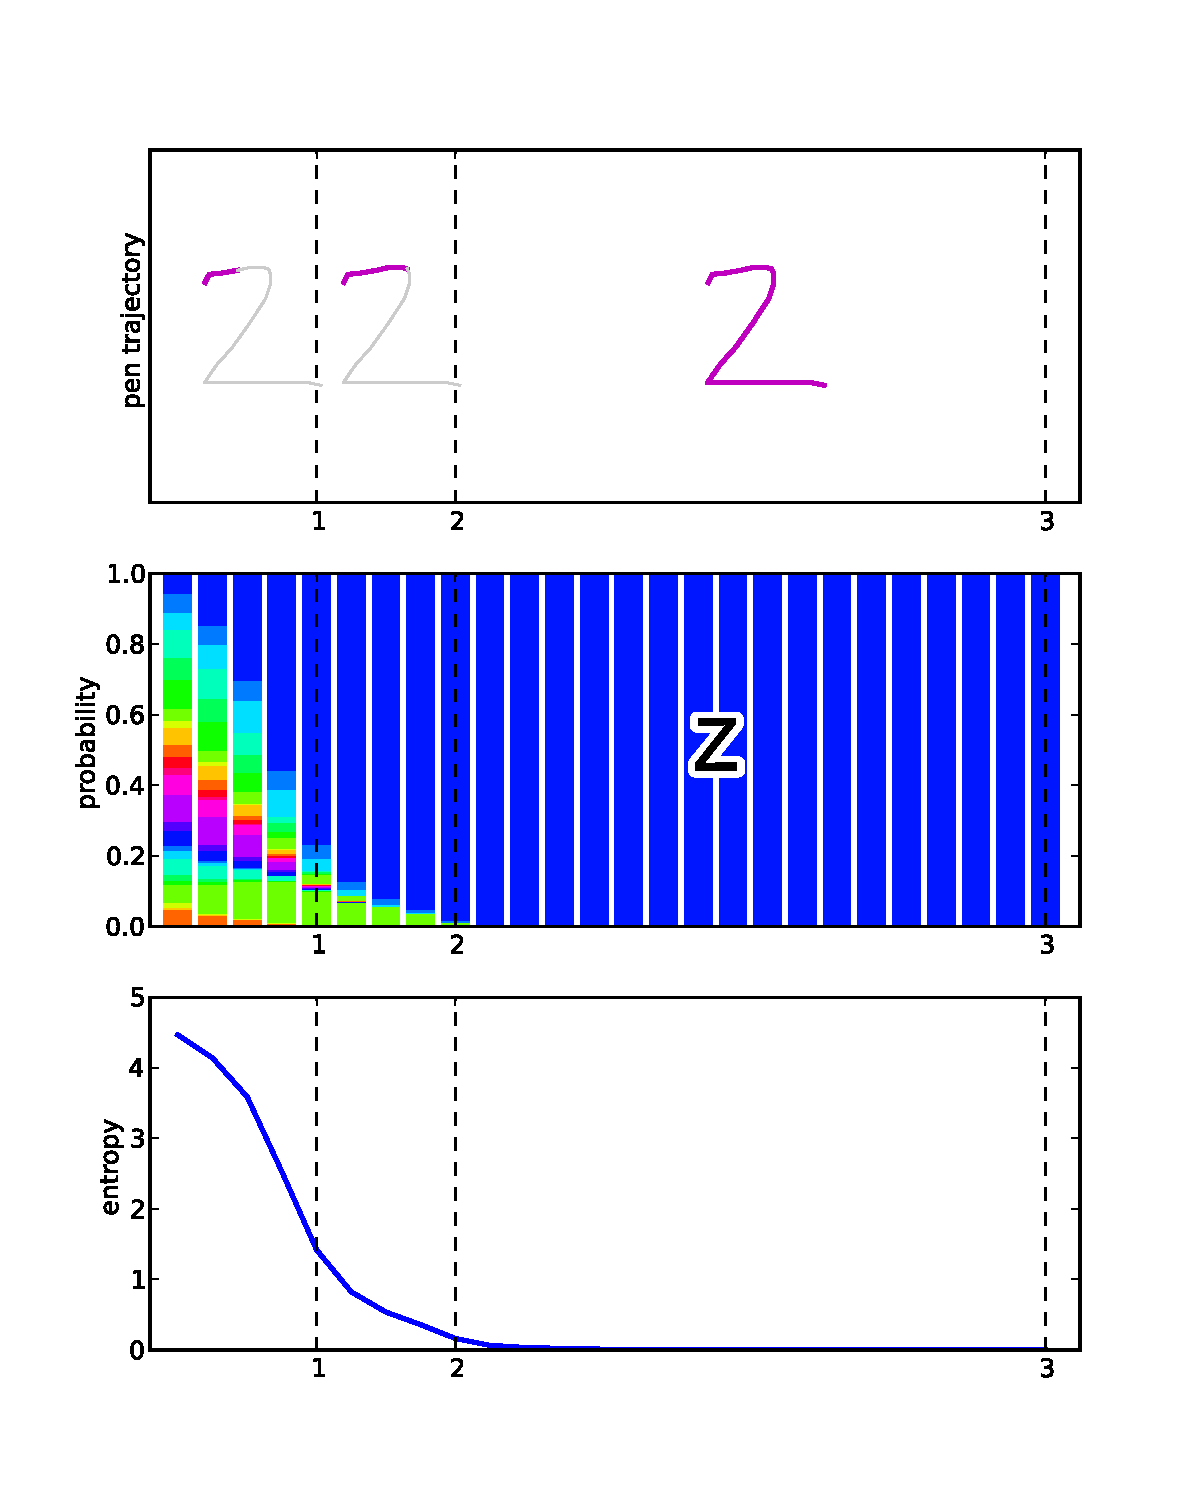
\includegraphics[width=\textwidth]{figures/entropy_z.pdf}
    \caption{}
    \label{fig:entropy_z}
  \end{subfigure}
  \begin{subfigure}[b]{0.45\textwidth}
    \begin{tabular}{c}
      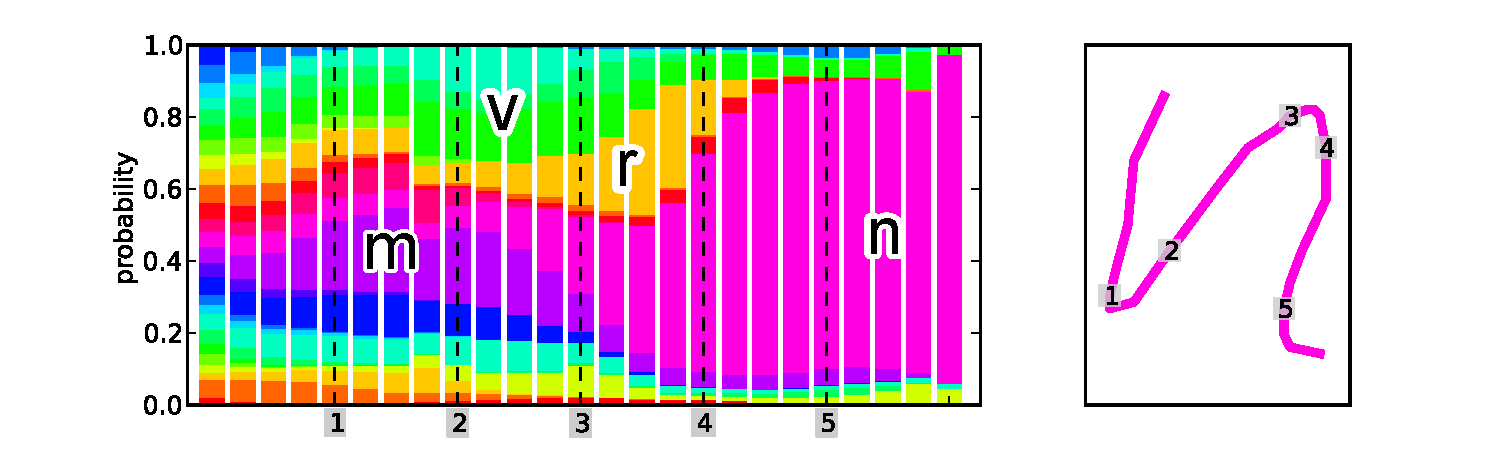
\includegraphics[width=\textwidth]{figures/best_l1.pdf}\\
      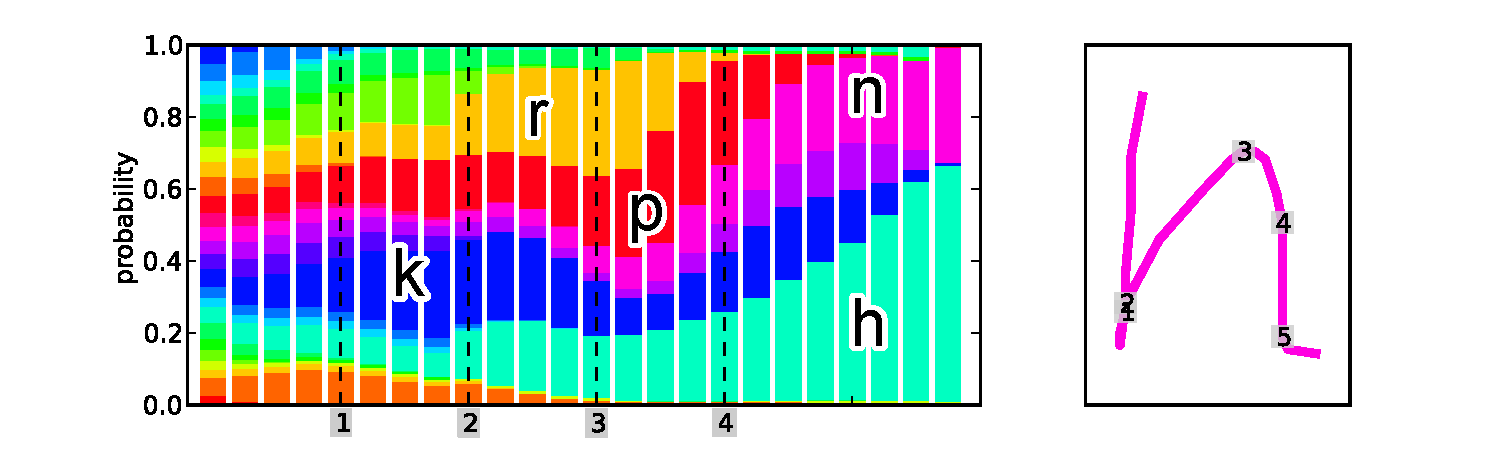
\includegraphics[width=\textwidth]{figures/unclear_l1.pdf}\\
      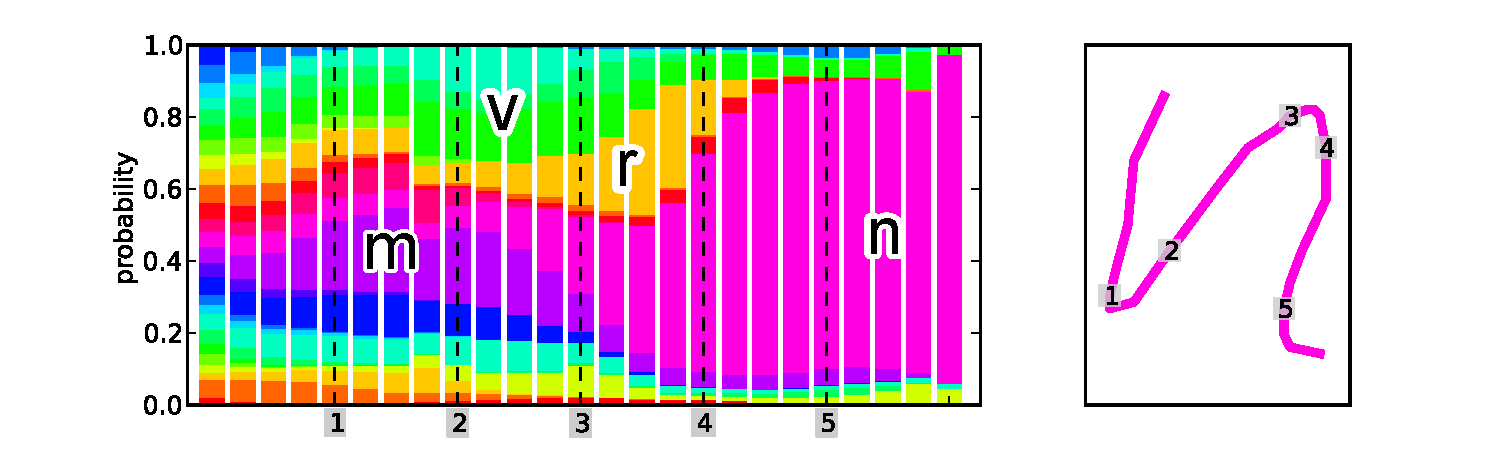
\includegraphics[width=\textwidth]{figures/best_l2.pdf}
    \end{tabular}
    \caption{}
    \label{fig:confusion}
  \end{subfigure}
  \caption{The conditional entropy $\condEntropy$ quickly reduces to 0
    when there is no confusion with other prototypes.  --- Three
    handwritten examples from a single user. The top example and the
    bottom example are recognized correctly as an 'n' and an 'h'
    respectively. The middle example is recognized as an 'h' instead
    of the true label 'n'.}
\end{figure}

In Figure~\ref{fig:confusion}, we show the posterior distributions
over time of 3 examples selected from a single user: a correctly
recognized 'n', a correctly recognized 'h' and an 'n' that was
recognized as an 'h'. We notice that, when the system correctly
recognized an 'n', the probability of 'n' increases significantly
between \frame{2} and \frame{4}, which corresponds to the upward
movement of the hand when writing both 'n' and 'h'. This information
can be delivered to the user in a form of the instructional feedback
to encourage the user to pay more attention to the upward movement part
when writing the pair.

\begin{figure}
  \centering
  \begin{subfigure}[b]{0.25\textwidth}
    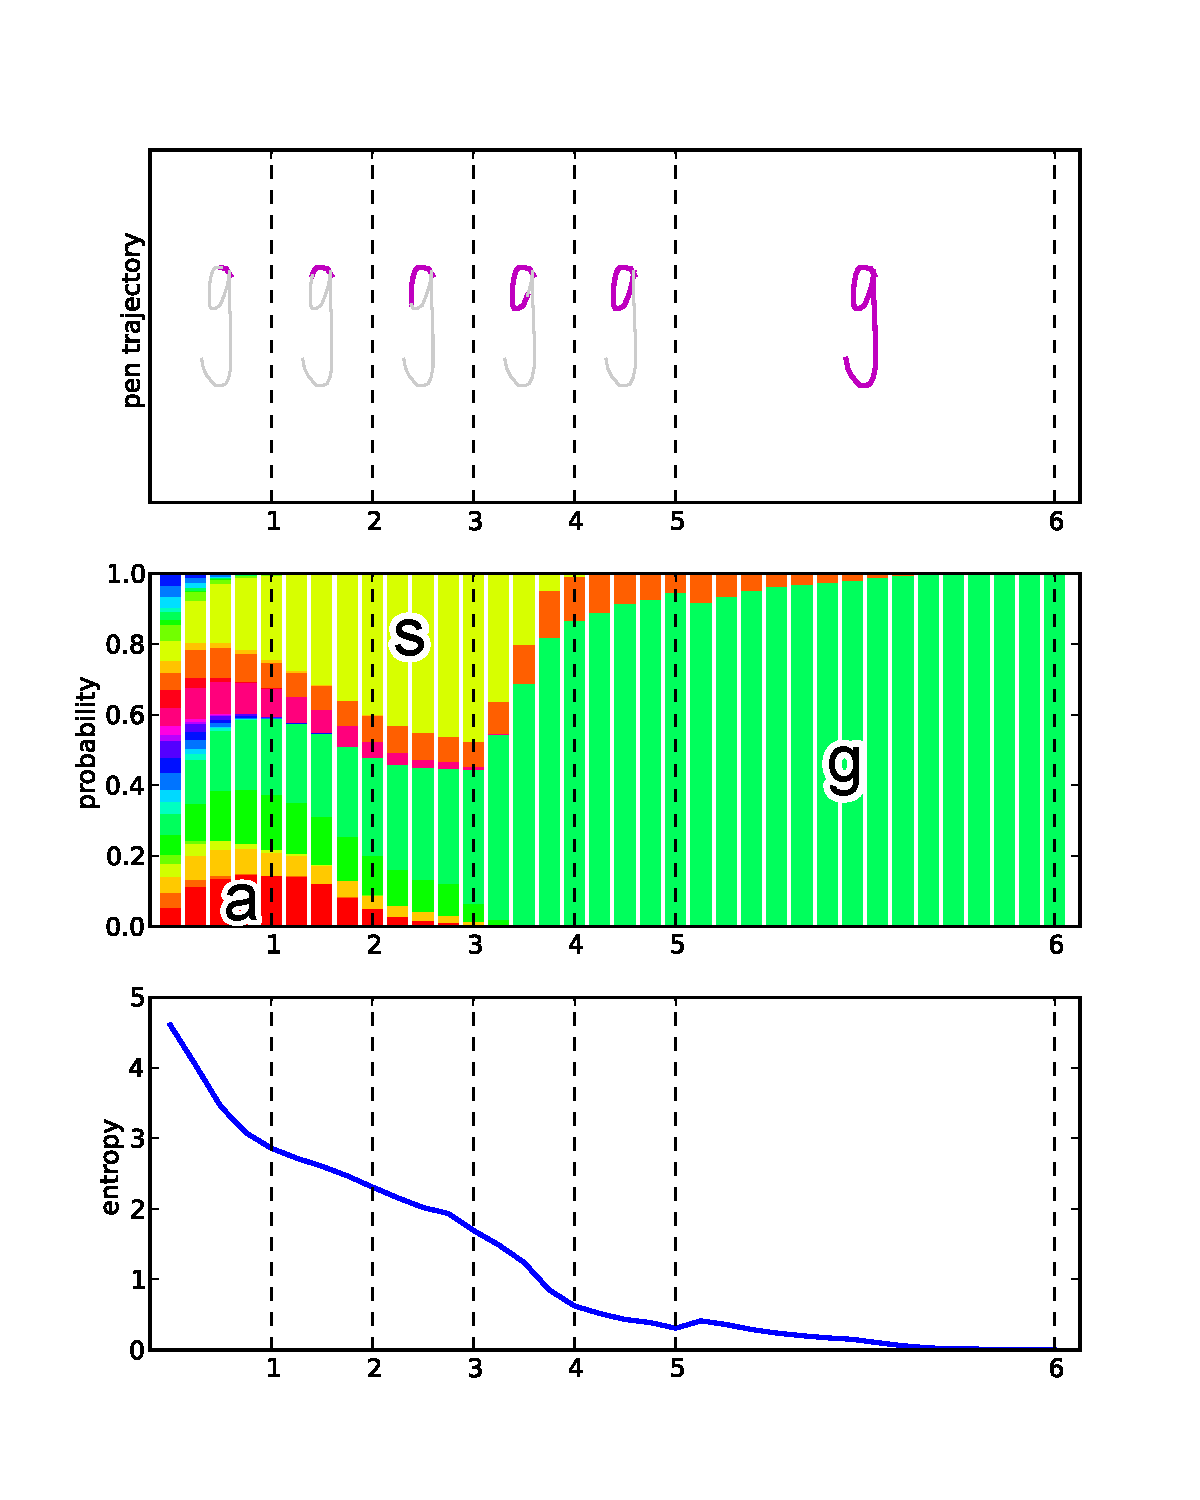
\includegraphics[width=\textwidth]{figures/entropy_g.pdf}
    \caption{}
    \label{fig:entropy_g}
  \end{subfigure}
  \begin{subfigure}[b]{0.25\textwidth}
    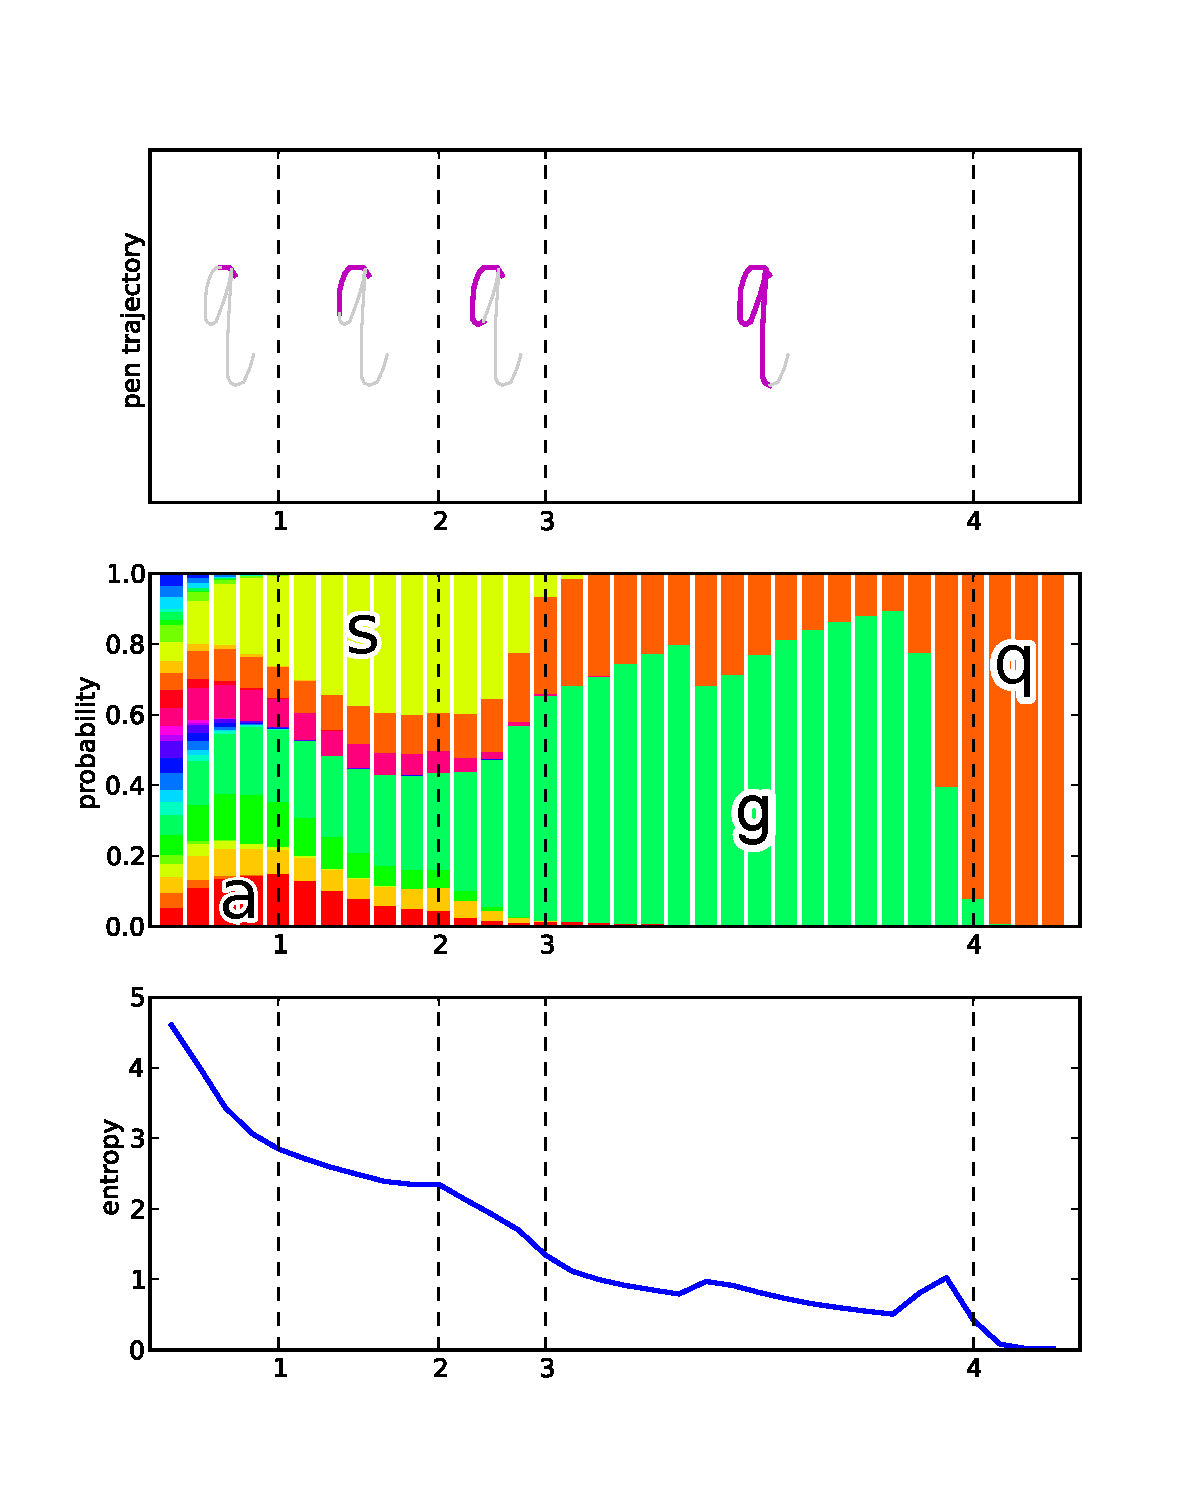
\includegraphics[width=\textwidth]{figures/entropy_q.pdf}
    \caption{}
    \label{fig:entropy_q}
  \end{subfigure}
  \begin{subfigure}[b]{0.25\textwidth}
    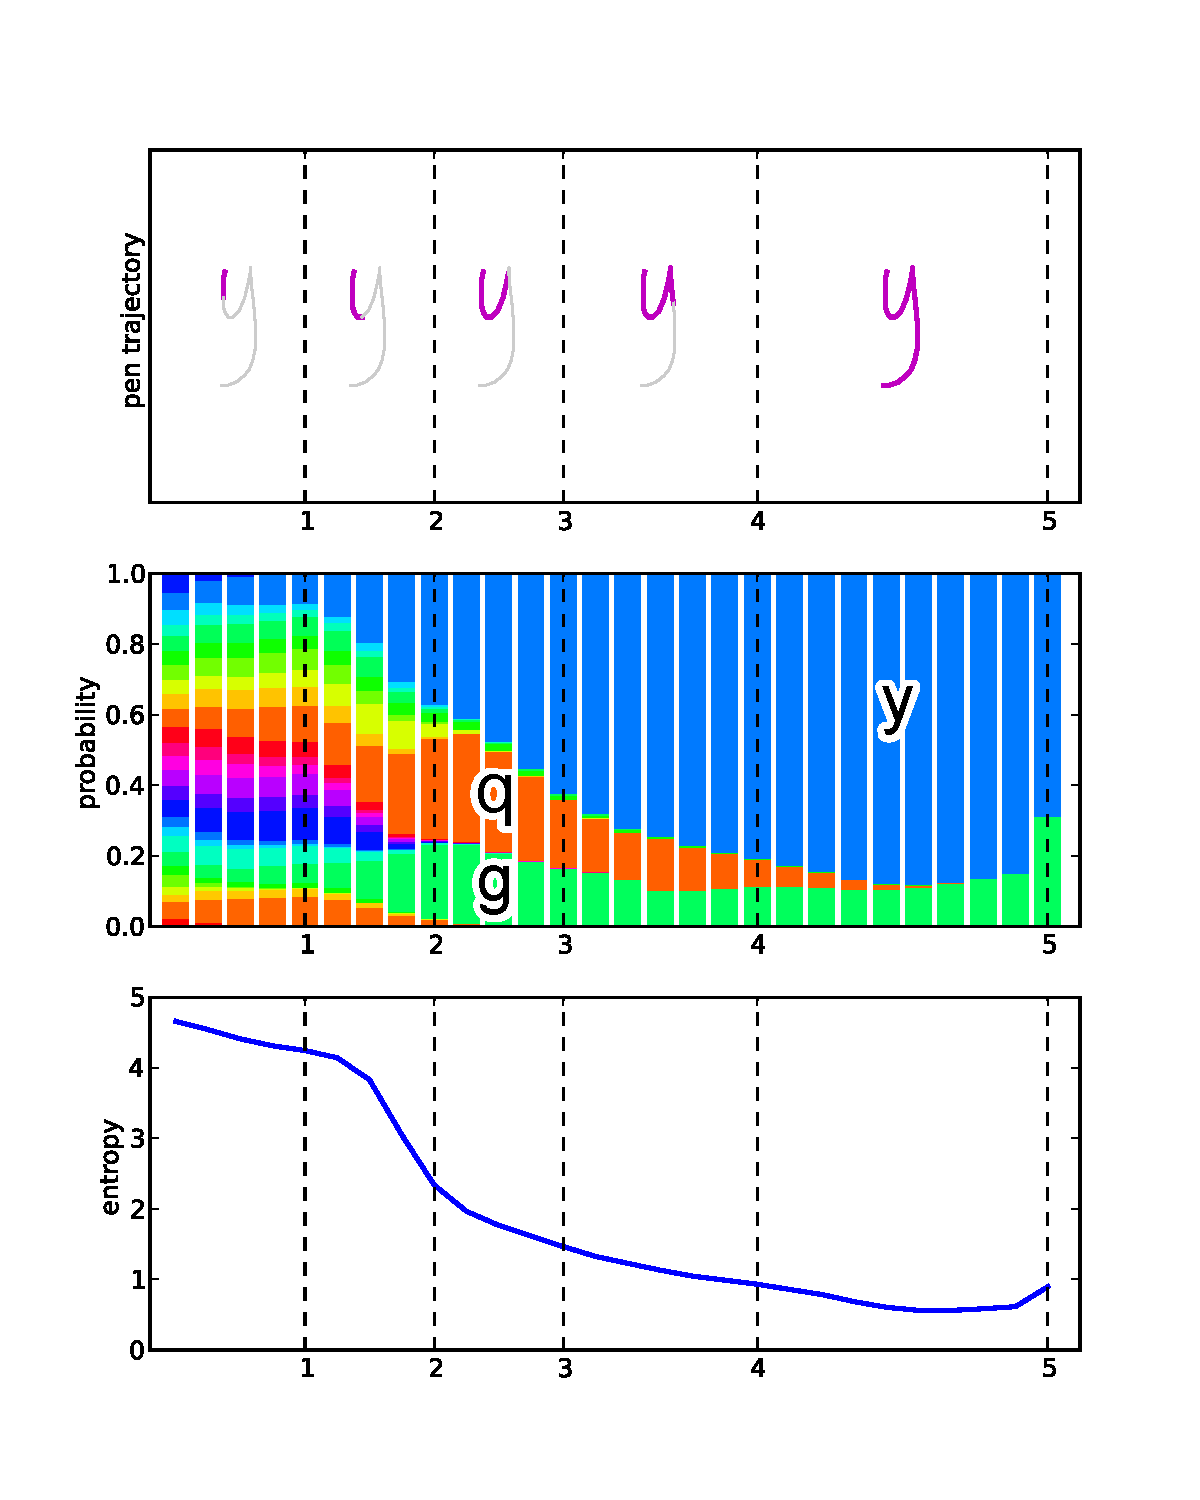
\includegraphics[width=\textwidth]{figures/entropy_y.pdf}
    \caption{}
    \label{fig:entropy_y}
  \end{subfigure}
  \caption{The posterior distributions as a function of time. The top
    row is the partial handwriting trajectories up to each dotted
    line. The middle row is the likelihood distributions over time
    where each color corresponds to each label. The bottom row is the
    entropy over time. }
  \label{fig:entropy}
\end{figure}


\section{Conclusions}
\label{sec:conclusions}

In this paper, we presented a theoretical framework for quantifying
the data transfer rate of a system that combines a human writer and a
handwriting recognition system. We developed an adaptative character
recognition algorithm and showed the results of a small deployment of
the system. From the results, we concluded that both the adaptation of
the computer (machine learning) and the adaptation of the human
(learning to write) needs to be considered together in order to design
a system that maximizes the information rate. Finally, we performed a
detailed analysis of the information transmission within the time a
single letter is written. Based on this analysis we can pinpoint the
location where the writer is failing to clearly disambiguate two
letters. On the other hand, we find other letters which are recognized
shortly after they begin. These identify inefficiencies in the coding
process and suggests ways we can teach the user to write in a way that
would increase the over channel rate of the system.




% Balancing columns in a ref list is a bit of a pain because you
% either use a hack like flushend or balance, or manually insert
% a column break.  http://www.tex.ac.uk/cgi-bin/texfaq2html?label=balance
% multicols doesn't work because we're already in two-column mode,
% and flushend isn't awesome, so I choose balance.  See this
% for more info: http://cs.brown.edu/system/software/latex/doc/balance.pdf
%
% Note that in a perfect world balance wants to be in the first
% column of the last page.
%
% If balance doesn't work for you, you can remove that and
% hard-code a column break into the bbl file right before you
% submit:
%
% http://stackoverflow.com/questions/2149854/how-to-manually-equalize-columns-
% in-an-ieee-paper-if-using-bibtex
%
% Or, just remove \balance and give up on balancing the last page.
%
\balance

% If you want to use smaller typesetting for the reference list,
% uncomment the following line:
% \small
\bibliographystyle{acm-sigchi}
\bibliography{iui-sunsern}
\end{document}
